\chapter{Final Notes and Conclusions}

In this chapter we will discuss the general conclusions of our work, as well as some observations that were made over the course of this project.
Whilst there were significant setbacks of our work -- chief among them being nearly two years of debugging, as well as a total refactoring of our work for a different hydrodynamical code -- the main goals of the project were completed.
Through this project we have developed a flexible and fast dust evolution code which can be used to simulate the growth of grains in numerical simulations of a WCd system.
Our dust model has been found to produce realistic yields of dust within both persistent and episodic dust forming CWB systems.
This is despite dust production not being artificially limited with orbital separation in the case of episodic WCd systems, while producing a similar degree of variability compared to observational studies of these systems.
Hysteresis of dust production is observed, which is also in-line with what is observed in episodic WCd systems.

Despite these successes, there is still much to add to this model.
More complex future models could incorporate additional dust growth and destruction mechanisms, and be more kinematically accurate.
WCd systems are still quite poorly known, and comparatively rare in the stellar catalogues.
However, more detailed studies of new and previously observed systems will be possible with the next generation of telescopes.

Whilst our dust production rates were typically on the order of what is expected for a WCd system, the production rate was underestimated in certain cases, in particular in the parameter space search.
This is most likely due to three factors:

\begin{itemize}
  \item Missing grain growth mechanisms, such as grain-grain collision.
  \item An incomplete grain nucleation model, which was out of the scope of this project.
  \item Conservative choices in model parameters, such as the grain sticking factor, $\xi$.
\end{itemize}

\noindent
As such, the bulk of this work was centred around qualitative research of the dust production of WCd systems.
Quantitative work would be preferable when undergoing future research with more advanced models.

\section{Conclusions}

In this section we will discuss the key conclusions of the papers published from this project, \emph{\firstpapertitle{}} and \emph{\secondpapertitle}.
In particular, we will discuss the changes in the production of dust in these systems as well as how these matched with our predictions and observational findings.

\subsection{Causes of dust growth in WCd systems}

In our first paper, \emph{\firstpapertitle}, we explore the system parameters thought to affect dust growth and dust production rates within WCd systems.
The system parameters that were studied were:

\begin{itemize}
  \item The mass loss rate, $\mdot$.
  \item The wind terminal velocity, $\vinf$.
  \item The orbital separation distance between the stars, $\dsep$.
\end{itemize}

\noindent
We conclude that while all of these parameters influenced the dust production rates of the system, two of the parameters had an outsized influence on production.
Modifying the wind terminal velocity of either star resulted in a significant increase or decrease in the dust production rate.
We observed a change in the dust production rate by as much as six orders of magnitude between the most and least prolific dust forming systems.
Slow dense winds have more radiative, cooler WCRs, which are more conducive to dust production.
However, we also observed that systems with a fast secondary wind can also drive significant dust production, despite not containing significant quantities of dust.
This suggests that in addition to cooling, the ratio of the wind velocities plays an important role in dust production, as an increased shear drives KH instabilities.
We also find that the change in orbital separation, $d\rms{sep}$ also significantly changes the dust production rate.
Closer orbits result in a significantly increased dust production rate.
This is due to a higher wind density upon collision, resulting in stronger post-shock cooling.

One of the key underlying factors of dust production -- in addition to cooling -- appears to be due to the formation of instabilities of either the KH or radiative thin-shell types.
As the wind parameter, $\chi$, decreases, we begin to observe rapid cooling in the WCR, as well as the presence of instabilities.
We also observe the aforementioned KH instabilities from velocity shear.
These instabilities result in the formation of high density clumps of cool, post-shock wind.
These clumps then form significant quantities of dust, which were observed when comparing the density to the dust-to-gas mass ratios of the simulations.

Whilst varying the stellar mass loss rates can contribute to a change in dust production rate, this is for the most part due to an increased initial grain number density.
However, an increased mass loss rate for either star can result in both more gas that can be converted to dust, as well as stronger shocks, leading to more cooling.

\subsection{The role of eccentricity in dust formation}

In our second paper: \emph{\secondpapertitle}, we confirmed that the dust production is significantly influenced by a continuously changing orbital separation.
% Clear points
This is in line with observations of WR140 at periastron, as well as our predictions from our previously published paper.
Part of the orbit around periastron was simulated, as dust production was anticipated to be greatest there.
Dust yields were found to be sensible, albeit higher than the average dust production rates predicted by \textcite{lauRevisitingImpactDust2020}, due to this limited simulation range.

% Hysteresis
Dust production also shows a degree of hysteresis.
The maximum dust production rate of the system occurs shortly after periastron passage.
This is partially due to the travel time between the stars to the WCR, which is on the order of a few days.
The maxima is reached extremely rapidly, and as the stars recede from each other, we find that the dust production rate tapers off slowly.
This is expected based on observations of characteristic carbon dust emission lines, where we see a similar tapering of the $L^\prime$ emission of WR140 \parencite{crowther_dust_2003}.
It was also observed that the time taken for the system to cease producing dust was similar to the time taken for the observed $L^\prime$ flux to diminish to regular levels.
Finally, we observe that even after the simulation should be behaving adiabatically, there is significant post-shock WCR cooling and instabilities, which encourage the production of dust.

% Orbital radial velocity
Some part of this hysteresis is due to the radial velocity of the system.
As we have found in our previous paper, WCd systems dust production rates are extremely dependent on the wind pre-shock velocity.
An increase in radial velocity as the stars approach periastron will increase the perceived wind velocity relative to the WCR.
As such, there is a corresponding decrease in the dust formation rate; the inverse is true as the stars recede from one another.
This velocity variability was found to be on the order of \SI{160}{km.s^{-1}}, suggesting it is not the primary reason for the asymmetry in the rate of dust production.
% This is not reflected in our model, but could be a contributing factor in the prolonged dust producing phase of the real WR140 system.


\subsubsection{Radiative driving}

Radiative line driving was not modelled in any simulations in this work.
Whilst this may not significantly change the results of the research in Chapter \ref{chap:parameterspace}, it could be the case that the wind velocity of the secondary star is lower than anticipated.
Analysing the single wind outflow of each star in the system we find that the wind velocity is reduced to 84\% of the expected amount.
% Based on our results, this would somewhat lower the dust production at periastron, due to a decreased velocity shear.
Whilst this would somewhat lower the dust production at periastron by reducing $\chi$ and reducing the wind velocity shear (though the latter is most likely a secondary effect).
This discrepancy is most likely smaller than the influence due to the conservative value for the grain sticking factor, $\xi$.
However, this would be a useful consideration in future models, especially when simulating systems which extremely close periastron passages.

\section{Future Study}

As we have frequently discussed throughout this thesis, there are still many things to cover in this field.
Some potential future avenues of research will be discussed, categorised into theoretical or observational research, as well as whether they are a short-term or long-term project.

\subsection{More complex models}

Our dust model, \bidmas{}, is designed to be comparatively flexible and extensible.
Additional dust growth and destruction mechanisms could be included; such as grain-grain collision and photoevaporation.
Long-term goals would be significant rewriting of the dust model in order to incorporate a multi-fluid dust grain model that is coupled to the gas through drag forces.
This would behave similarly to \textcite{hendrix_pinwheels_2016}, though with grain growth, destruction and cooling.
This would be useful as the velocities between gas and dust grains could be better calculated, allowing for more accurate growth and destruction rates.
This extended model could also be used to simulate dust mixing within the post-shock WCR.
As dust has significantly more inertia than the medium it is travelling through, it could be the case that dust grains could enter the secondary, hydrogen rich OB flow, which could affect grain growth, and allow for complex chemical models. 

A dust grain nucleation model could also be implemented, in order to better determine the initial conditions of the system -- and therefore make more quantitative evaluations of these systems.
% This would also obviate the need to assume that the relative grain number density is constant throughout a simulation.
Finally, a chemical model could also be included, though this would take significant work\ldots

\subsection{Further simulations of observed systems}

A deeper parameter search of the effect of modifying wind terminal velocity for each star was considered, but there was insufficient time to complete the simulations and analyse the data before the end of the PhD.
Deriving a fuller relation between dust production and $\vinf$ for both systems would be a useful near-term project.
A similar study for orbital separation using a wider range of orbits, or system eccentricities could also be performed.
Simulation of other systems that were considered for this project such as WR104 would also be an additional significant near-term goal.
Qualitative studies of these systems would be easier to implement, compared to broader parameter space studies.
However, AMR would be required in order to simulate these systems, due to their close-in or distant orbits, which do not favour the refinement conditions of SMR.
The main limiting factor to simulating systems is having well known wind parameters and orbital parameters.
As large telescopes are built and more detailed surveys of WCd systems are performed, more of these systems will become amenable to simulation in the future.

\subsection{Radiative transfer}

Another future project could be the use of an IR radiative transfer code such as \texttt{HYPERION} \parencite{robitailleHYPERIONOpensourceParallelized2011} to generate synthetic observations of the systems being simulated.
Whilst this was an initial goal of the project, there was little time to modify the in-house radiative transfer code to calculate IR emissivities instead of x-ray and radio.
There was also insufficient time to study these systems using open source codes.
This is similar to research conducted by \textcite{hendrix_pinwheels_2016}, and would allow the gap to be bridged between our numerical studies and observational studies of these systems.
This research could also be performed in conjunction with research into these systems from newer telescope arrays that have not been used to observe these systems, such as ALMA.

\subsection{WR+WR systems}

Another topic of extreme interest is WR+WR systems like Apep (Section \ref{sec:bg-apep}) and WR48a (Section \ref{sec:bg-wr48a}).
% Rarity, reasons for this, improb. 
So far, only two such systems have been confirmed.
They are predicted to be quite rare due to the improbability of both stars being in their short lived WR phases at the same time.
% Dust production rates, distances
These systems, while having tremendous total mass loss rates, do not produce significant quantities of dust.
This is quite curious, though it may be potentially due to their comparatively similar wind velocities and wide overall separation (though the orbital elements are still quite uncertain, see \cite{hanExtremeCollidingwindSystem2020}), if we are to extrapolate from our current results.
% Metallicities, WN/WC
The presence of another hydrogen depleted wind, such as that of an WN sequence WR star would result in interesting conditions for the systems, such as both winds being highly radiative.
% Eccentricities in orbits
Both systems are found to be quite eccentric, with the orbital period of Apep being \SI{125(20)}{\year} \parencite{hanExtremeCollidingwindSystem2020}.
This also may explain their comparatively low dust production rates.
% More data needed, more systems needed, statistically very rare
More data is needed to properly assess these systems, however.
% Extragalactic sources, LMC/SMC?
Extra-galactic systems could also be potentially simulated, with best-guess values for their orbital and wind parameters.
Comparison of these systems with galactic systems could also present an interesting avenue of research.

\subsection{\emph{Telescopes: The Next Generation}}

\begin{figure}
  \centering
  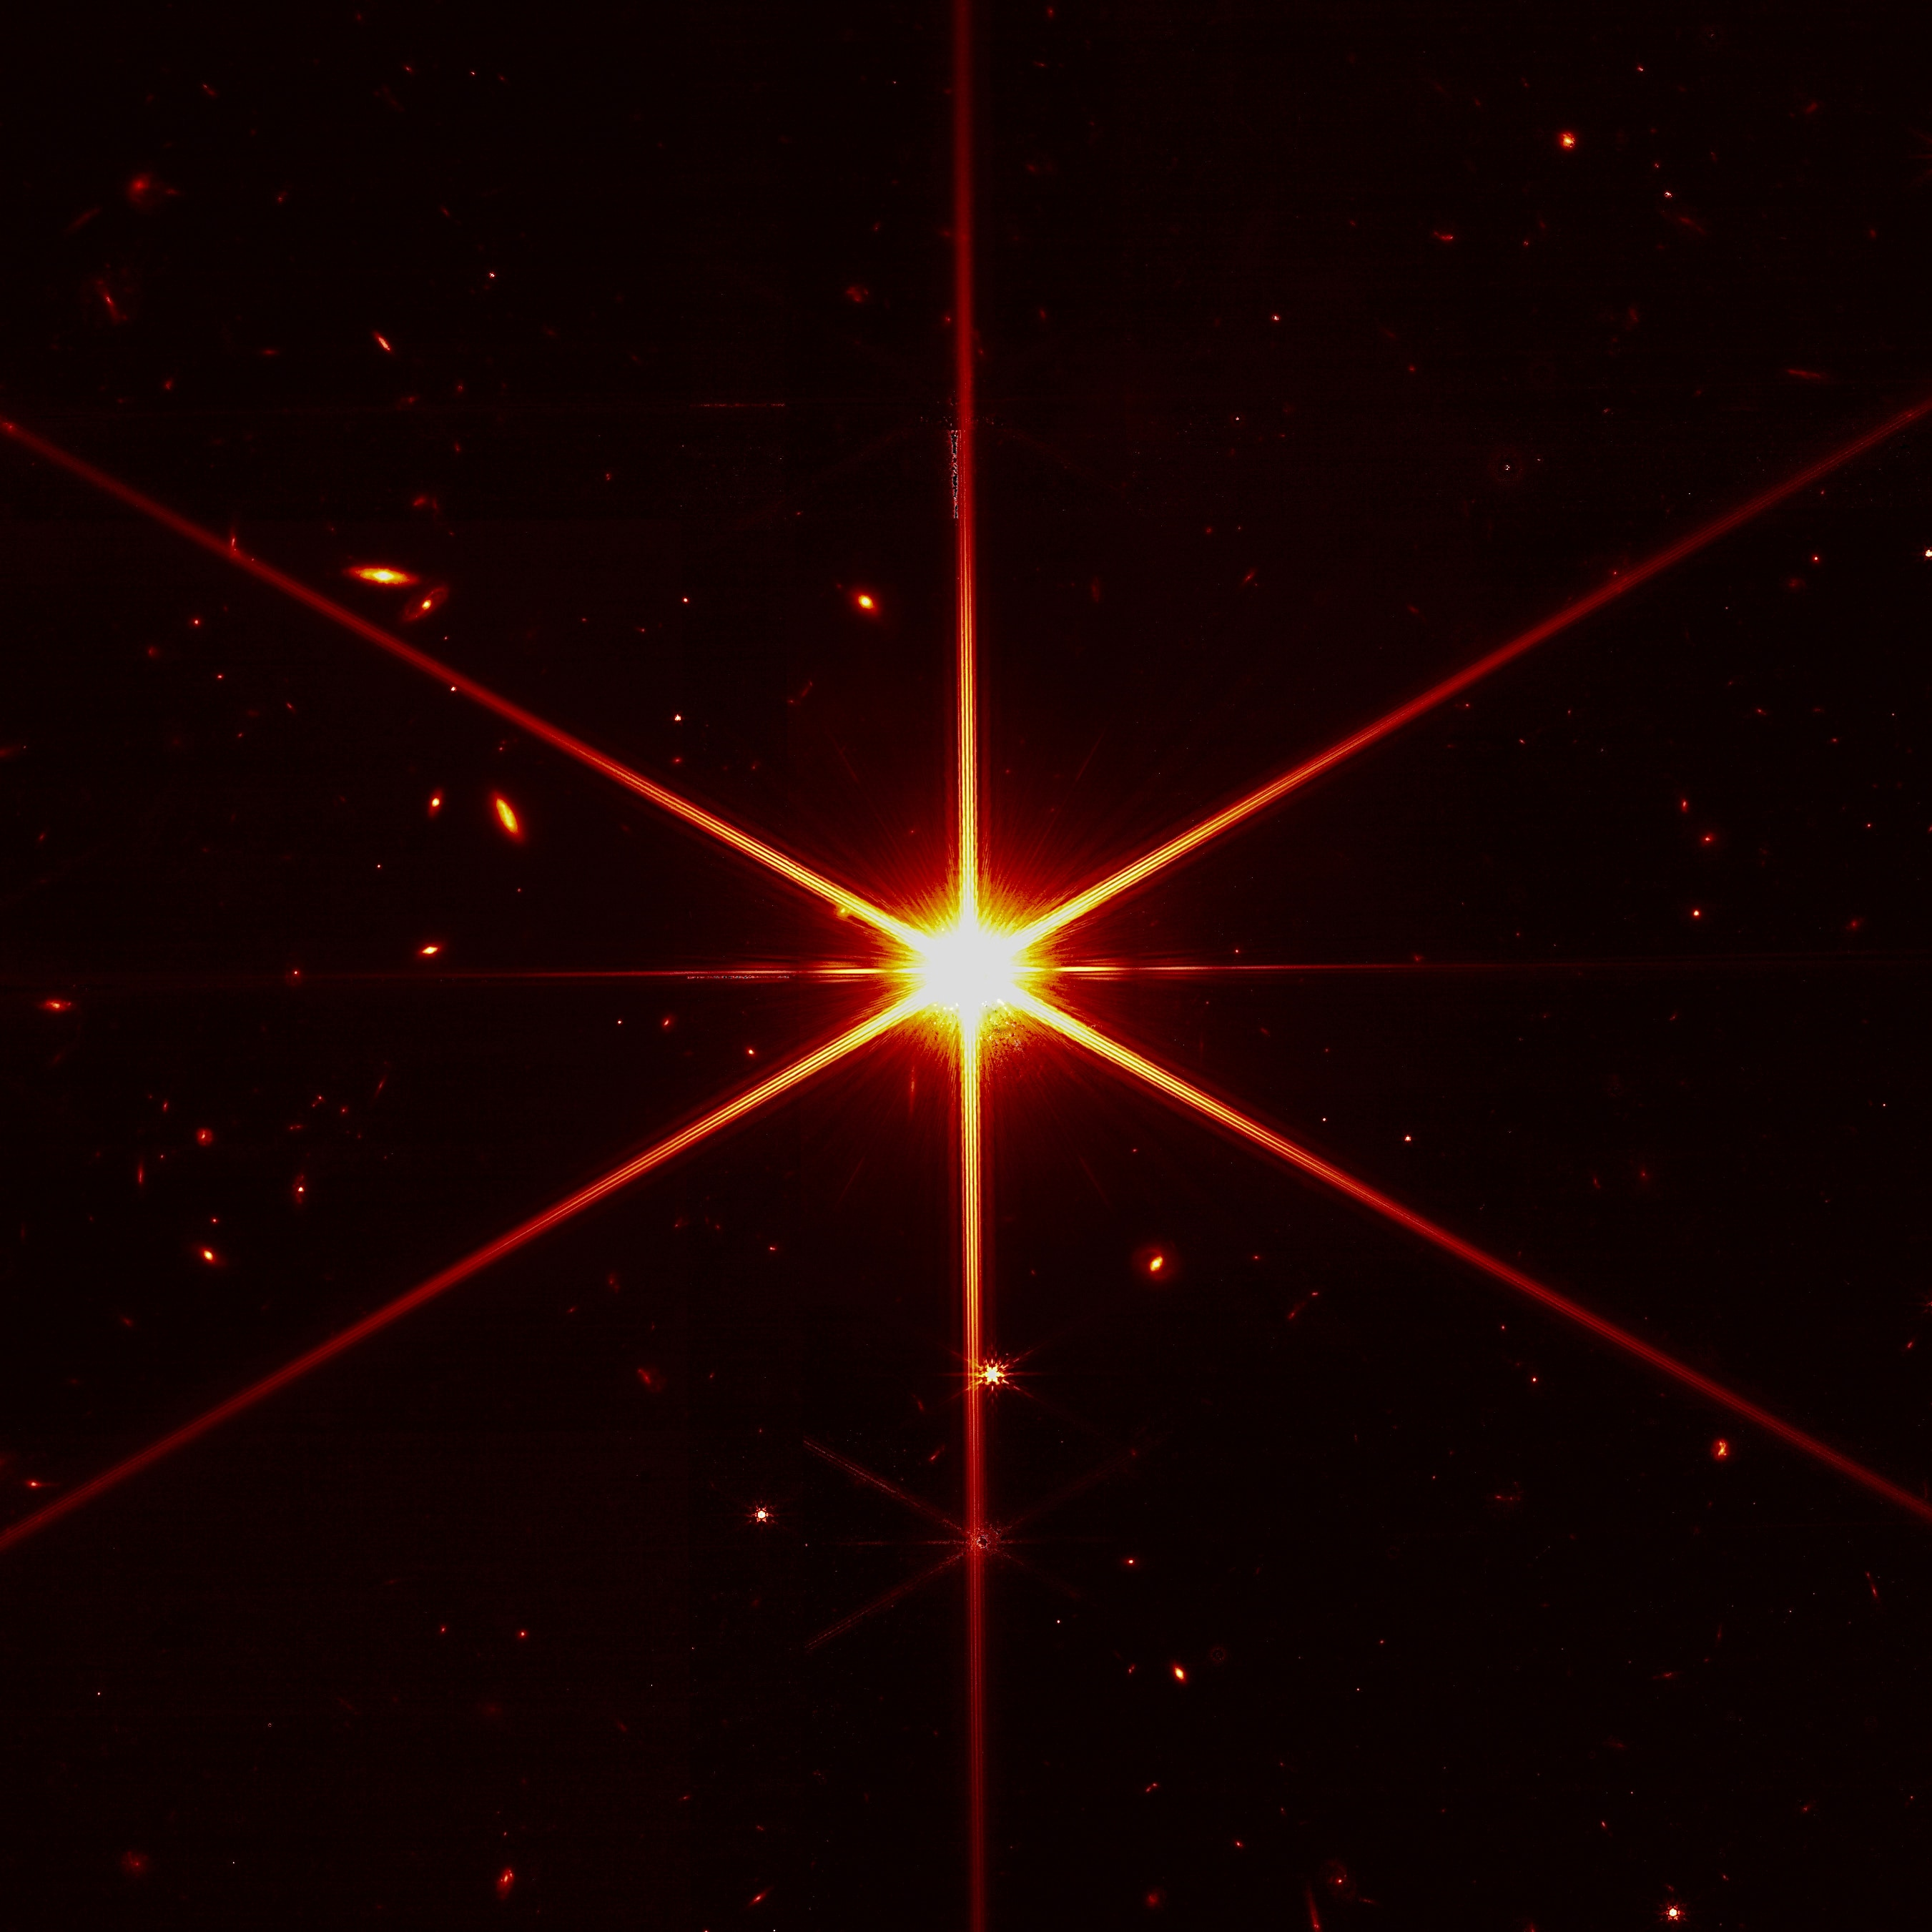
\includegraphics[width=3in]{assets/jwst.jpg}
  \caption[First telescope alignment evaluation image from the JWST]{First telescope alignment evaluation image from the JWST. Despite the initial alignment performing better than expected, we are still months away from scientific observations, and perhaps years away from observing WCd systems.}
  \label{fig:jwst}
\end{figure}

% JWST 
The James Webb Space Telescope (JWST; Fig. \ref{fig:jwst}) represents the pinnacle of the observational sciences.
% Nail biting
From a nail biting launch to month-long deployment, I'm sure it is safe to say that many astrophysicists were more than a little bit nervous throughout the month of December.
But now, the mirrors are aligned and cooling, and scientific observation is due to commence within the next few months -- we can all breathe a sigh of relief.
JWST is uniquely well-suited to observing these systems, due to its incredible sensitivity, high angular resolution and near/mid-IR spectral range.
Additionally, extremely high sensitivity spectrographic observation from JWST would help determine orbits and wind compositions to a greater degree of accuracy.
Ground based arrays such as ALMA could also perform this, especially as instrumentation such as ALMA band 2 come online.
% Luvoir
Other future space-based telescopes, like the spiritual successor to the Hubble, the Luvoir telescope, could overcome the difficulties of observing WCd systems.
Though this would not be for a number of decades.
Astronomy is -- as many of us know -- occasionally a waiting game\ldots


\section{Other Observations}

This short section covers other, more personal observations made throughout this PhD.

\subsection[\textit{How I Learned to Stop Worrying and Love Numerics}]{\textit{Doctorate Strangelove or: How I Learned to Stop Worrying and Love Numerics}}

Numerical simulation is an extremely complex topic, and when things go wrong, it can be enormously time consuming and sanity testing to fix.
Sometimes code that works fine on one platform being used for testing will not run correctly, or refuse to compile at all.
On occasion it felt like the software paradigm of WOCA\footnote{Write Once, Compile Anywhere.} simply did not apply when writing in allegedly portable languages, such as \texttt{C}.
The code is also difficult to debug and fix, due to the performance impact, and being essentially unable to set breakpoints unless the simulation crashes within the first timestep.

Simulation work is difficult, and often frustrating, but is extremely satisfying when things begin to go right.
On top of that, being able to run dozens of simulations on parallel on HPC resources meant that an entire parameter space search could be performed simultaneously, something that isn't possible in observational work.
As such, once the model was finished, running simulations took approximately 4 months in total, not including analysis.
Based on experiences other researchers I have talked to who undertook simulation-based work, this is a fairly common experience.

\subsection{Become a researcher, see the world!}

Between the issues in our earlier attempts to get our model to work correctly in the \mg{} hydrodynamical code, to a personal injury to the current global pandemic
(see Section \ref{sec:pandemic}), to the simple unavailability of relevant conferences, no conferences were attended throughout this project.
I'm sure (especially considering the pandemic) that many other researchers are or have been in the same boat, though it is a considerable shame.

I look forward to any future conference that I may visit in my academic career.

\subsection{Paul Erd\H{o}s was probably onto something}

The second half of my PhD represented for the first time in my life that I was consistently treating my ADHD with medication.
Whilst this made me nervous initially, I found myself for the first time being able to think \emph{clearly}.
To those who don't know, there are few things quite as frustrating as finding yourself completely, utterly unable to work because you simply can't think clearly or keep on topic.
In fact, I'm not confident I would have been able to finish this PhD without a small amount of (prescribed) chemical assistance.

The sheer difference in the amount and consistency of my work after I began medicating made me think of a quote from the mathematician Paul Erd\H{o}s.
After successfully quitting cold turkey from amphetamines for a month after a bet with his colleague Ronald Graham, he said this to him as he collected his \$500:

\begin{quote}
  \emph{
  \noindent
  ``You've showed me I'm not an addict. But I didn't get any work done. I'd get up in the morning and stare at a blank piece of paper. I'd have no ideas, just like an ordinary person. You've set mathematics back a month.''
  }
\end{quote}

\noindent
In closing, if you, the reader, empathise with this\ldots{} It might be a good idea to get yourself checked.

\subsection{Carinae Strain: PhD research in a time of pandemic}
\label{sec:pandemic}

Whilst the world outside was terrifying, and everything seemed like it was only going to get worse during the pandemic lockdowns, it is hard to stay motivated about anything.
But there truly is nothing more helpful and calming than enjoying a show or a game with your friends and loved ones, even if it is over the internet rather than in person.

\begin{center}
  Thank you, everyone, for helping me through this.
\end{center}

\section{The Last Word}

This thesis demonstrates the effectiveness of an advected scalar dust model to estimate the yields of dust produced in a WCd system.
We also use this model to quantitatively evaluate how various system parameters and behaviours change the growth rate of dust in the system.
We find two system parameters in particular to be particularly important to the production of dust, $\vinf$ and $\dsep$.
Subsequently, we conclude that the episodic nature of some WCd systems is due to their eccentric orbits.
% The presence of instabilities appears to be very conducive to dust production, and hysteresis has been observed in these instabilities, leading to a slow reduction in dust production rate as an eccentric WCd system passes periastron.
Continued development of the model and further observational work is essential to better understanding WCd systems.
Due to many difficulties throughout the project, there was limited time to include a fully comprehensive dust model composed of a separate, coupled fluid.
Other avenues of research include synthetic imaging through radiative transfer, as well as improved observations and surveys using next-generation telescopes.
WCd systems represent a tremendous scientific curiosity still, in particular how the initial nascent grains form and survive in these systems.

As my supervisor wrote when ending his thesis:

\begin{center}
  \emph{``There remains much work to be done\ldots''}
\end{center}